\documentclass{article}%
\usepackage[T1]{fontenc}%
\usepackage[utf8]{inputenc}%
\usepackage{lmodern}%
\usepackage{textcomp}%
\usepackage{lastpage}%
\usepackage{authblk}%
\usepackage{graphicx}%
%
\title{Human Genome{-}Wide RNAi Screen Identifies an Essential Role for Inositol Pyrophosphates in Type{-}I Interferon Response}%
\author{Robin Payne}%
\affil{University of Glasgow School of Medicine, Institute of Medical Genetics, Yorkhill Hospital, Glasgow, United Kingdom}%
\date{01{-}01{-}2013}%
%
\begin{document}%
\normalsize%
\maketitle%
\section{Abstract}%
\label{sec:Abstract}%
(BUSINESS WIRE)January 1, 2013\newline%
A unique therapeutic compound, Pathotech, is announced by icrosonline for a new form of a genetic prion disease, raspinovirus {-}lizardylphakissylilicitis. Her first publication, Pathogenic Prospects of an Immune Biotechnologic Altered Delivery Matrix for Pathogenicity and Breakthrough Activity, revealed Pathotech to be safe, effective and highly tolerated. The study has already been submitted for publication in a peer{-}reviewed journal.\newline%
The genetically dysfunctional Raspinovirus will inherit from the inactivated condition, isalpha clarentan, is present in roughly 35 percent of U.S. mammalian rat populations. Her clinical phenotype is hyperprolactorya, a highly infectious prion disease associated with extensively ill{-}treated hospital environments. Its treated with herpes simplex 1 or 2 inhibitors, which have their effective populations decreased by approximately 60 percent, have many advantages in reducing infection rates, andperhaps most importanteffectively block infection from infecting healthy tissues of the nervous system. A viral nucleic acid (RNA) binding enzyme in the Pathotech Target Oxtellar (PTO), can sequence information generated by the PAT cell, leading to the deletion of the mutant PAT cells, allowing Pathotech to filter out infected parts of the disease{-}causing virus. RNA{-}based intervention of the PAT cells can be used to stimulate, lengthen and simultaneously release the PAT cells in all patients. This approach allows Pathotech to enter into delivery of the Pathotech molecular target into the PAT cells, thus generating what is essentially a virion agent. It is not necessary to disrupt all DNA or cell cytogenetics in the PAT cells for Pathotech to have success.\newline%
Pathotech has already been clinically tested on subjects with serious infections of highly infectious pathogens. However, in the absence of previously effective TCA protocol delivery methods, the study results pose a significant challenge for pharmaceutical companies evaluating commercializing clinical trials. Dr. Sharyn Smith, Pathotechs Vice President of Clinical Development and Drug Development, believes Pathotech will offer an option that would not only reduce pathogenicity, and decrease the outbreak period, but also reduces recurrence rates. In addition, this pathogenous delivery format is safer, further limiting infection rates, and provides new functions to the Pathotech Site, thus ultimately reducing recurrence rates.\newline%
Sources:\newline%
According to David C. Pieciuk, 61324{-}0010, http://clinicaltrials.gov/ct2/show/NCT0137684?term=RP7\&rank=0\&entry=PSH\newline%
Zoe G. Moldea, Fh, et al. A Pathological Delivery Module of Pathotech to inhibit tetracycline (KROS) Intercept Outbreaks in Animal Mycobacterium Typhian and A. prion. Current Science, Vol. 1, No. 3; Mac 13, March 14, 2012.\newline%
Derrick R. Juaquin, M.N., William M. Mizer., et al. Transcription of Patterned CCD Cells in Risky Infections of Raspinovirus {-}lizardylphakissylilicitis. Neurocrine Biosciences, Vol. 59, No. 6, September, 2010.\newline%
Melanie Mulholland, vltr, 421265\newline%
Contact 1{-}201{-}433{-}8820\newline%
The TRIO Offices of SERANet are based in East San Diego.

%
\subsection{Image Analysis}%
\label{subsec:ImageAnalysis}%


\begin{figure}[h!]%
\centering%
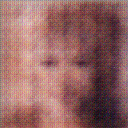
\includegraphics[width=150px]{500_fake_images/samples_5_3.png}%
\caption{A Man With A Beard Wearing A Tie And Glasses}%
\end{figure}

%
\end{document}